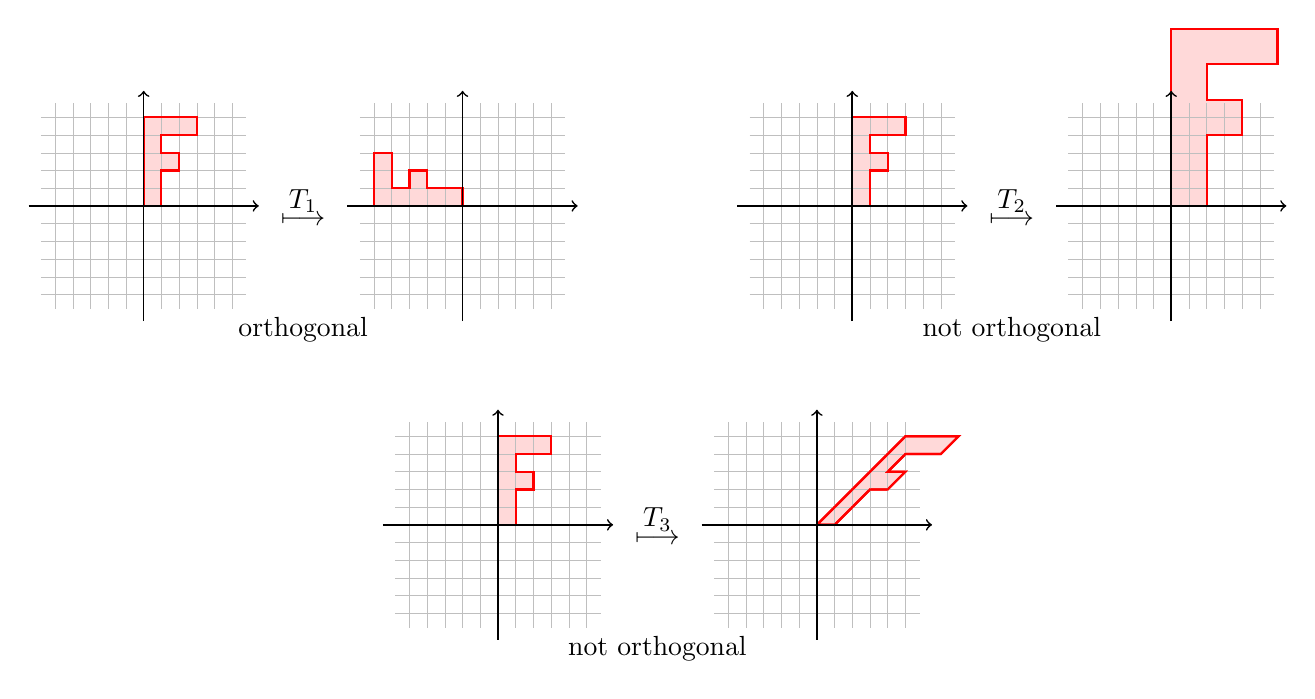
\begin{tikzpicture}[scale=0.9]
      \begin{scope}
        \begin{scope}[scale=0.25]
          \draw[red,thick,fill=red!15]
          (0,0) -- (0,5) -- (3,5) -- (3,4) -- (1,4) --
          (1,3) -- (2,3) -- (2,2) -- (1,2) -- (1,0) -- cycle;
          \draw[step=1cm, gray!50, very thin] (-5.8,-5.8) grid (5.8,5.8);
          \draw[red,thick]
          (0,0) -- (0,5) -- (3,5) -- (3,4) -- (1,4) --
          (1,3) -- (2,3) -- (2,2) -- (1,2) -- (1,0) -- cycle;
          \draw[semithick,->] (-6.5,0) -- (6.5,0);
          \draw[semithick,->] (0,-6.5) -- (0,6.5);
        \end{scope}
        \begin{scope}[xshift=2.25cm]
          \path (0,0) node {$\stackrel{\displaystyle T_1}{\longmapsto}$};
          \path (0,-1.75) node {orthogonal};
        \end{scope}
        \begin{scope}[xshift=4.5cm,scale=0.25]
          \draw[red,thick,fill=red!15,cm={0,1,-1,0,(0,0)}]
          (0,0) -- (0,5) -- (3,5) -- (3,4) -- (1,4) --
          (1,3) -- (2,3) -- (2,2) -- (1,2) -- (1,0) -- cycle;
          \draw[step=1cm, gray!50, very thin] (-5.8,-5.8) grid (5.8,5.8);
          \draw[red,thick,cm={0,1,-1,0,(0,0)}]
          (0,0) -- (0,5) -- (3,5) -- (3,4) -- (1,4) --
          (1,3) -- (2,3) -- (2,2) -- (1,2) -- (1,0) -- cycle;
          \draw[semithick,->] (-6.5,0) -- (6.5,0);
          \draw[semithick,->] (0,-6.5) -- (0,6.5);
        \end{scope}
      \end{scope}
      \begin{scope}[xshift=10cm]
        \begin{scope}[scale=0.25]
          \draw[red,thick,fill=red!15]
          (0,0) -- (0,5) -- (3,5) -- (3,4) -- (1,4) --
          (1,3) -- (2,3) -- (2,2) -- (1,2) -- (1,0) -- cycle;
          \draw[step=1cm, gray!50, very thin] (-5.8,-5.8) grid (5.8,5.8);
          \draw[red,thick]
          (0,0) -- (0,5) -- (3,5) -- (3,4) -- (1,4) --
          (1,3) -- (2,3) -- (2,2) -- (1,2) -- (1,0) -- cycle;
          \draw[semithick,->] (-6.5,0) -- (6.5,0);
          \draw[semithick,->] (0,-6.5) -- (0,6.5);
        \end{scope}
        \begin{scope}[xshift=2.25cm]
          \path (0,0) node {$\stackrel{\displaystyle T_2}{\longmapsto}$};
          \path (0,-1.75) node {not orthogonal};
        \end{scope}
        \begin{scope}[xshift=4.5cm,scale=0.25]
          \draw[red,thick,fill=red!15,cm={2,0,0,2,(0,0)}]
          (0,0) -- (0,5) -- (3,5) -- (3,4) -- (1,4) --
          (1,3) -- (2,3) -- (2,2) -- (1,2) -- (1,0) -- cycle;
          \draw[step=1cm, gray!50, very thin] (-5.8,-5.8) grid (5.8,5.8);
          \draw[red,thick,cm={2,0,0,2,(0,0)}]
          (0,0) -- (0,5) -- (3,5) -- (3,4) -- (1,4) --
          (1,3) -- (2,3) -- (2,2) -- (1,2) -- (1,0) -- cycle;
          \draw[semithick,->] (-6.5,0) -- (6.5,0);
          \draw[semithick,->] (0,-6.5) -- (0,6.5);
        \end{scope}
      \end{scope}
      \begin{scope}[xshift=5cm,yshift=-4.5cm]
        \begin{scope}[scale=0.25]
          \draw[red,thick,fill=red!15]
          (0,0) -- (0,5) -- (3,5) -- (3,4) -- (1,4) --
          (1,3) -- (2,3) -- (2,2) -- (1,2) -- (1,0) -- cycle;
          \draw[step=1cm, gray!50, very thin] (-5.8,-5.8) grid (5.8,5.8);
          \draw[red,thick]
          (0,0) -- (0,5) -- (3,5) -- (3,4) -- (1,4) --
          (1,3) -- (2,3) -- (2,2) -- (1,2) -- (1,0) -- cycle;
          \draw[semithick,->] (-6.5,0) -- (6.5,0);
          \draw[semithick,->] (0,-6.5) -- (0,6.5);
        \end{scope}
        \begin{scope}[xshift=2.25cm]
          \path (0,0) node {$\stackrel{\displaystyle T_3}{\longmapsto}$};
          \path (0,-1.75) node {not orthogonal};
        \end{scope}
        \begin{scope}[xshift=4.5cm,scale=0.25]
          \draw[red,thick,fill=red!15,cm={1,0,1,1,(0,0)}]
          (0,0) -- (0,5) -- (3,5) -- (3,4) -- (1,4) --
          (1,3) -- (2,3) -- (2,2) -- (1,2) -- (1,0) -- cycle;
          \draw[step=1cm, gray!50, very thin] (-5.8,-5.8) grid (5.8,5.8);
          \draw[red,thick,cm={1,0,1,1,(0,0)}]
          (0,0) -- (0,5) -- (3,5) -- (3,4) -- (1,4) --
          (1,3) -- (2,3) -- (2,2) -- (1,2) -- (1,0) -- cycle;
          \draw[semithick,->] (-6.5,0) -- (6.5,0);
          \draw[semithick,->] (0,-6.5) -- (0,6.5);
        \end{scope}
      \end{scope}
    \end{tikzpicture}
